\documentclass[tikz,border=4pt]{standalone}

\usepackage{amsmath}
\usetikzlibrary{arrows.meta}

\begin{document}

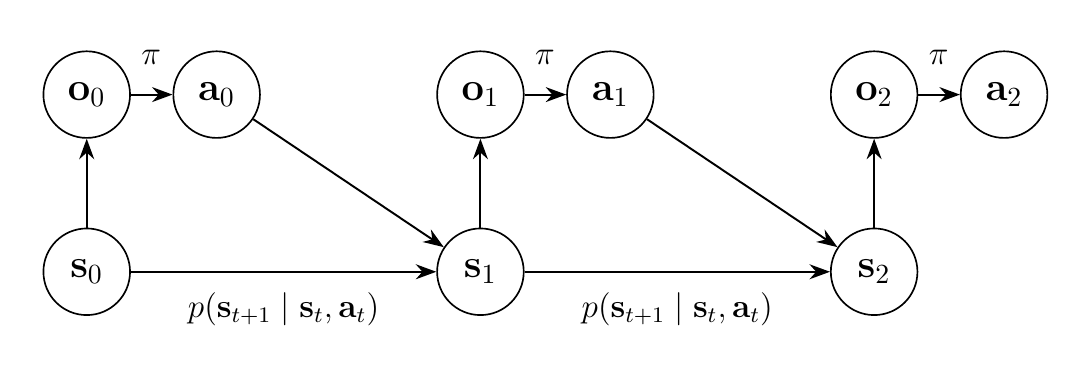
\begin{tikzpicture}[
  node/.style={
    circle,
    draw,
    line width=0.6pt,
    minimum size=11mm,
    inner sep=0pt,
    font=\Large
  },
  edge/.style={
    -{Stealth[length=2.6mm,width=1.9mm]},
    line width=0.7pt
  },
  label/.style={
    inner sep=1.3pt
  }
]

\path[use as bounding box] (-0.75,-0.90) rectangle (12.30,3.10);

\node[node] (s0) at (0,0) {$\mathbf{s}_0$};
\node[node] (s1) at (5.0,0) {$\mathbf{s}_1$};
\node[node] (s2) at (10.0,0) {$\mathbf{s}_2$};
\node[node] (a0) at (1.65,2.25) {$\mathbf{a}_0$};
\node[node] (a1) at (6.65,2.25) {$\mathbf{a}_1$};

\node[node] (o0) at (0,2.25) {$\mathbf{o}_0$};
\node[node] (o1) at (5.0,2.25) {$\mathbf{o}_1$};
\node[node] (o2) at (10.0,2.25) {$\mathbf{o}_2$};
\node[node] (a2) at (11.65,2.25) {$\mathbf{a}_2$};

\draw[edge] (s0) -- (o0);
\draw[edge] (o0) -- (a0);
\draw[edge] (a0) -- (s1);
\draw[edge] (s0) -- (s1);

\draw[edge] (s1) -- (o1);
\draw[edge] (o1) -- (a1);
\draw[edge] (a1) -- (s2);
\draw[edge] (s1) -- (s2);

\draw[edge] (s2) -- (o2);
\draw[edge] (o2) -- (a2);

\node[label, font=\large] at (0.82,2.72) {$\pi$};
\node[label, font=\large] at (5.82,2.72) {$\pi$};
\node[label, font=\large] at (10.82,2.72) {$\pi$};

\node[label, font=\large] at (2.50,-0.48)
  {$p(\mathbf{s}_{t+1}\mid\mathbf{s}_t,\mathbf{a}_t)$};
\node[label, font=\large] at (7.50,-0.48)
  {$p(\mathbf{s}_{t+1}\mid\mathbf{s}_t,\mathbf{a}_t)$};

\end{tikzpicture}

\end{document}
